% das Papierformat zuerst
%\documentclass[a4paper, 11pt]{article}

% deutsche Silbentrennung
%\usepackage[ngerman]{babel}

% wegen deutschen Umlauten
%\usepackage[ansinew]{inputenc}

% hier beginnt das Dokument
%\begin{document}


\thispagestyle{empty}

%\begin{figure}[t]
% \includegraphics[width=0.6\textwidth]{abb/fh_koeln_logo}
%\end{figure}

\begin{figure}[t]
 \centering
 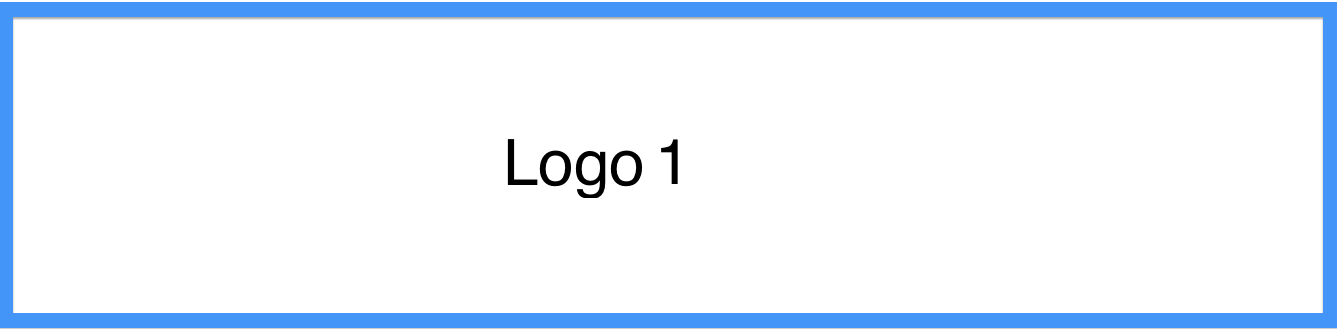
\includegraphics[width=0.6\textwidth]{abb/logo1}
~~~~~~~~~~
 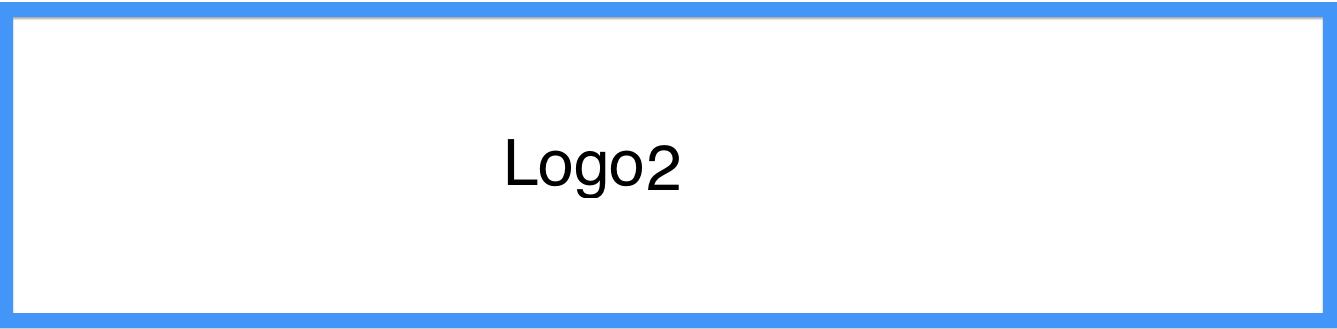
\includegraphics[width=0.20\textwidth]{abb/logo2}
\end{figure}


\begin{verbatim}


\end{verbatim}

\begin{center}
\Large{University of Bayreuth}\\
\end{center}


\begin{center}
\Large{Department of Informatics}
\end{center}
\begin{verbatim}








\end{verbatim}
\begin{center}
\doublespacing
\textbf{\LARGE{\titleDocument}}\\
\singlespacing
\begin{verbatim}

\end{verbatim}
\textbf{{~\subjectDocument}}
\end{center}
\begin{verbatim}

\end{verbatim}
\begin{center}

\end{center}
\begin{verbatim}






\end{verbatim}
\begin{flushleft}
\begin{tabular}{llll}
\textbf{Topic:} & & Integration of JPA-conform ORM-Implementations & \\
	& & in Hibernate Search & \\
& & \\
\textbf{Author:} & & Martin Braun <martinbraun123@aol.com>& \\
& & Matrikel-Nr. 1249080 & \\
& & \\
\textbf{Version date:} & & \today &\\
& & \\
\textbf{1. Supervisor:} & & Prof. Dr. Stefan Jablonski &\\
\textbf{2. Supervisor:} & & Prof. Dr. Bernhard Westfechtel &\\
\end{tabular}
\end{flushleft}